\documentclass{article}

\usepackage{amsmath}
\usepackage{amsfonts} 
\usepackage{geometry}
\usepackage{multicol}
\usepackage{float}
% \usepackage{mathtools}
% \usepackage{graphicx}
% \usepackage{soul}
% \usepackage{indentfirst}
\usepackage{tikz}
\usetikzlibrary{calc, automata, chains, arrows.meta, math}
\setcounter{MaxMatrixCols}{20}


\title{A game theoretic model of the behavioural gaming that takes place at the EMS - ED interface}

\author{
    Michalis Panayides, 
    Paul Harper, 
    Vince Knight
}

\begin{document}

\maketitle

\begin{abstract}
    The main focus of this research is the construction of a 3-player game theoretic model between two queueing systems and a service that distributes individuals to them. The resultant model will then be used to explore dynamics between all players.
    
    The first aspect of this work is the development of a queueing system with two consecutive waiting spaces. The strategic managerial behaviour corresponds to how individuals use these waiting spaces. Two modelling techniques were used: discrete event simulation and Markov chains. The state probabilities of the Markov chain system have been used to extract the performance measures of the queueing model (e.g. mean time in each waiting room, mean number of individuals in each room, etc.).
    
    A 3-player game theoretic model is proposed between the two queueing systems and the service that distributes individuals to them. In particular this can be seen as a 2-player normal-form game where the utilities are determined by a third player with its own strategies and objectives. A backwards induction technique is used to get the utilities of the normal-form game between the two queueing systems.
    
    This particular system can be applied in a healthcare scenario where it captures the emergent behaviour between, for example, the Emergency Medical Service (EMS) and the Emergency Department (ED). This will be used to investigate the impact of target measures on patient welfare.
\end{abstract}




\newpage
\tableofcontents

\newpage
\section{Introduction - Motivation}

\newpage
\section{Overview of game theoretic model}

\begin{figure}[h]
    \centering
    \begin{tikzpicture}[-, node distance = 3cm, auto]
        \node[anchor=north](H1){\(H_1\)};
        \node[anchor=north](H1_d1) at (3, 2){.};
        \node[anchor=north](H1_d2) at (3, -2){.};

        \path(H1) edge node {}(H1_d1);
        \path(H1) edge node {}(H1_d2);
        \path(H1_d1) edge [bend left] node {}(H1_d2);
        \path(H1_d1) [dashed] edge node {}(H1_d2);

        \node[anchor=north](H2) at (3.9, 0){\(H_2\)};
        \node[anchor=north](H2_d1) at (6.9, 2){.};
        \node[anchor=north](H2_d2) at (6.9, -2){.};

        \path(H2) edge node {}(H2_d1);
        \path(H2) edge node {}(H2_d2);
        \path(H2_d1) edge [bend left] node {}(H2_d2);

        \node[anchor=north](A) at (7.8, 0){\(A\)};
        \node[anchor=north](A_d1) at (10.8, 2){.};
        \node[anchor=north](A_d2) at (10.8, -2){.};
        
        \path(A) edge node {}(A_d1);
        \path(A) edge node {}(A_d2);
        \path(A_d1) edge [bend left] node {}(A_d2);

    \end{tikzpicture}
    \caption{Ambulance Decision Problem} 
    \label{Ambulance_Problem}
\end{figure}

\noindent 
{\Large\textbf{States:}}
\begin{enumerate}
    \item \(A\) = Ambulance
    \item \(H_i\) = Hospital i
\end{enumerate}

\noindent 
{\Large\textbf{Notation:}}
\begin{itemize}
    \item \(\Lambda\) = total number of patients that need to be hospitalised
    \item \(p_i\) = proportion of patients going to Hospital i (\(p_i\Lambda\) 
    = number of patients going to hospital i)
    \item \(\hat{c_i}\) = capacity of hospital i
    \item \(W(c, \lambda\, \mu)\) = waiting time in the system function
    \item \(\mu_i\) = service rate of hospital i
    \item \(\lambda_i^o\) = arrival rate of other patients to the hospital 
    (not by ambulance)
    \item \(C_i(p_i) = d_i + W(c = \hat{c_i},\hspace{0.1cm} \lambda = 
    p_i\Lambda + \lambda_i^o, \hspace{0.1cm} \mu = \mu_i)\)
\end{itemize}

\noindent 
{\Large\textbf{Players:}}
\begin{itemize}
    \item Ambulance
    \item Hospital A
    \item Hospital B
\end{itemize}

\noindent 
{\Large\textbf{Strategies of players:}}
\begin{itemize}
    \item Hospital i:    
    \begin{enumerate} 
        \item Close doors at \(\hat{c_i} = 1\) 
        \item Close doors at \(\hat{c_i} = 2\)
        \item \dots
        \item Close doors at \(\hat{c_i} = C_i\)
    \end{enumerate}
    \item Ambulance:
    \begin{enumerate}
        \item Choose \(p_1 \in [0,1]\) 
    \end{enumerate}
\end{itemize}

\noindent 
{\Large\textbf{Cost Function:}} Probability of waiting time less than target. 






\newpage
\section{A queueing model with 2 consecutive buffer centres}

\subsection{System}
The following Markov chain represents the transition between states of a service
centre 
while capturing the interactions between it and a buffer centre.
The service centre accepts two types of individuals; Class 1 and Class 2.  
Class 2 individuals are accepted until a pre-determined threshold \(T\) of 
individuals is reached.
When reached, all Class 2 individuals that arrive will remain \textit{``blocked''}
in the buffer centre until the number of people in the system is 
reduced below \(T\). 
Additionally, if the people in the service centre keep rising, they may exceed
the number 
of servers \(C\) available, which will in turn mean that every new person will 
have to wait for a server to become free. 
The states of the Markov chain are denoted by \((u,v)\) where:

\begin{itemize}
    \item \(u\) = number of Class 2 individuals blocked
    \item \(v\) = number of Class 1 individuals in the service centre
\end{itemize}

\begin{figure}
    \centering
    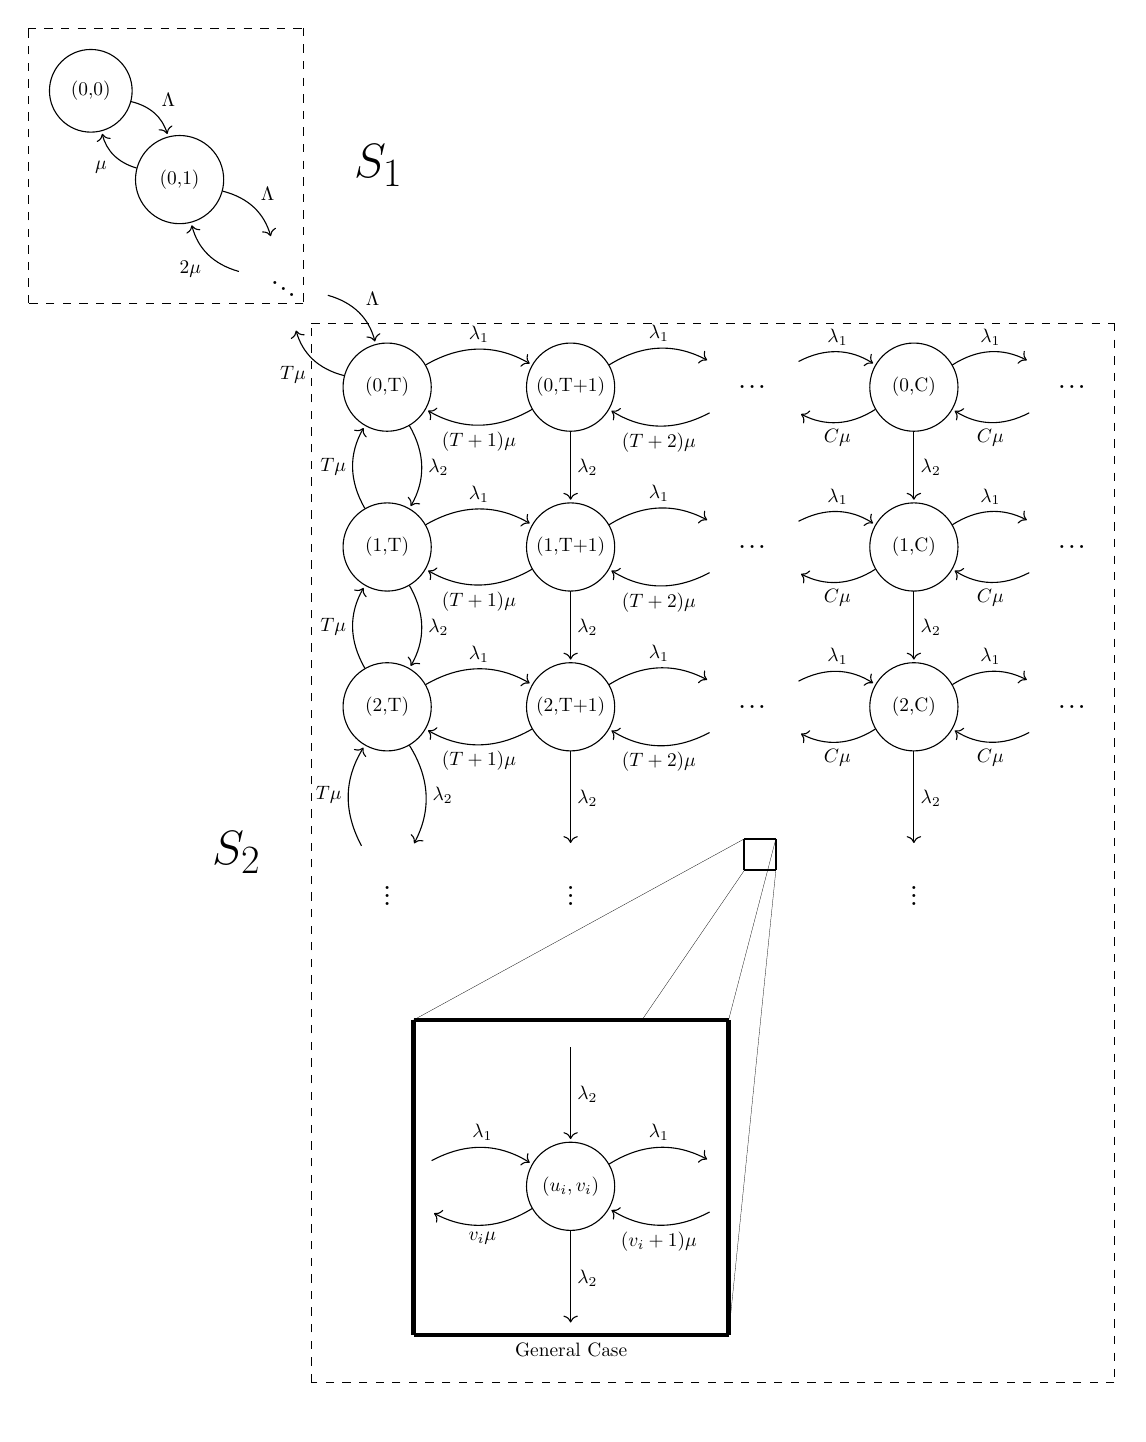
\begin{tikzpicture}[-, node distance = 0.9cm, auto, every node/.style={scale=0.7}]

        % Markov chain variables
        \tikzmath{
            let \initdist = 0.5cm;
            let \altdist = 1.2cm;
            let \minsz = 1.6cm;
        }

        % S_1 and S_2 rectangles
        \tikzmath{
            let \leftOne = -0.8;
            let \rightOne = 2.7;
            let \upOne = 0.8;
            let \downOne = -2.7;
            let \leftTwo = 2.8;
            let \rightTwo = 13;
            let \upTwo = -2.95;
            let \downTwo = -16.4;
        }

        % General case variables
        \tikzmath{
            let \GCsmallx = 8.3;
            let \GCsmally = -9.5;
            let \GCbigx = 4.1;
            let \GCbigy = -11.8;
        }

        % Rectangle for S1
        \draw[ultra thin, dashed] (\leftOne, \downOne) -- (\leftOne, \upOne);
        \draw[ultra thin, dashed] (\leftOne, \upOne) -- (\rightOne, \upOne);
        \draw[ultra thin, dashed] (\rightOne, \upOne) -- node 
        {\Huge{\( \quad S_1 \)}}(\rightOne, \downOne);
        \draw[ultra thin, dashed] (\rightOne, \downOne) -- (\leftOne, \downOne);

        % Rectangle for S2
        \draw[ultra thin, dashed] (\leftTwo, \downTwo) -- node 
        {\Huge{\( S_2 \quad \)}}(\leftTwo, \upTwo);
        \draw[ultra thin, dashed] (\leftTwo, \upTwo) -- (\rightTwo, \upTwo);
        \draw[ultra thin, dashed] (\rightTwo, \upTwo) -- (\rightTwo, \downTwo);
        \draw[ultra thin, dashed] (\rightTwo, \downTwo) -- (\leftTwo, \downTwo);

        % Small square of general case
        \draw [thick] (\GCsmallx, \GCsmally) -- node {} 
        (\GCsmallx + 0.4, \GCsmally);
        \draw [thick] (\GCsmallx + 0.4, \GCsmally) -- node {} 
        (\GCsmallx + 0.4, \GCsmally - 0.4);
        \draw [thick] (\GCsmallx + 0.4, \GCsmally - 0.4) -- node {} 
        (\GCsmallx, \GCsmally - 0.4);
        \draw [thick] (\GCsmallx, \GCsmally - 0.4) -- node {} 
        (\GCsmallx, \GCsmally);


        % Dashed lines to from small square to big one 
        \draw [ultra thin] (\GCsmallx, \GCsmally) -- node {} 
        (\GCbigx, \GCbigy);
        \draw [ultra thin] (\GCsmallx + 0.4, \GCsmally) -- node {} 
        (\GCbigx + 4, \GCbigy);
        \draw [ultra thin] (\GCsmallx, \GCsmally - 0.4) -- node {} (7, \GCbigy);
        \draw [ultra thin] (\GCsmallx + 0.4, \GCsmally - 0.4) -- node {} 
        (\GCbigx + 4, \GCbigy - 4);
        
        % Big Square of general case
        \draw [ultra thick] (\GCbigx, \GCbigy) -- node {} (\GCbigx + 4, \GCbigy);
        \draw [ultra thick] (\GCbigx + 4, \GCbigy) -- node {} 
        (\GCbigx + 4, \GCbigy - 4);
        \draw [ultra thick] (\GCbigx + 4, \GCbigy - 4) -- node {General Case} 
        (\GCbigx, \GCbigy - 4);
        \draw [ultra thick] (\GCbigx, \GCbigy - 4) -- node {} (\GCbigx, \GCbigy);

        % First Line
        \node[state, minimum size=1.5cm] (zero) {(0,0)};
        \node[state, node distance = \initdist, minimum size=\minsz, below right=of zero] 
        (one) {(0,1)};
        \node[draw=none, node distance = \initdist, minimum size=\minsz, below right=of one] 
        (two) {\textbf{\( \ddots \)}};
        \node[state, node distance = \initdist, minimum size=\minsz, below right=of two] 
        (three) {(0,T)};
        \node[state, node distance = \altdist, minimum size=\minsz, right=of three] 
        (four) {(0,T+1)};
        \node[draw=none, node distance = \altdist, minimum size=\minsz, right=of four] 
        (five) {\textbf{\dots}};
        \node[state, minimum size=\minsz, right=of five] (six) {(0,C)};
        \node[draw=none, minimum size=\minsz, right=of six] (seven) {\textbf{\dots}};

        % Second Line
        \node[state, minimum size=\minsz, below=of three] (three_one) {(1,T)};
        \node[state, minimum size=\minsz, below=of four] (four_one) {(1,T+1)};
        \node[draw=none, minimum size=\minsz, below=of five] (five_one) {\textbf{\dots}};
        \node[state, minimum size=\minsz, right=of five_one] (six_one) {(1,C)};
        \node[draw=none, minimum size=\minsz, right=of six_one] (seven_one) {\textbf{\dots}};
        
        % Third Line
        \node[state, minimum size=\minsz, below=of three_one] (three_two) {(2,T)};
        \node[state, minimum size=\minsz, below=of four_one] (four_two) {(2,T+1)};
        \node[draw=none, minimum size=\minsz, below=of five_one] (five_two) 
        {\textbf{\dots}};
        \node[state, minimum size=\minsz, right=of five_two] (six_two) {(2,C)};
        \node[draw=none, minimum size=\minsz, right=of six_two] (seven_two) 
        {\textbf{\dots}};

        % Fourth line
        \node[draw=none, node distance = \altdist, minimum size=\minsz, below=of three_two] 
        (three_three) {\textbf{\vdots}};
        \node[draw=none, node distance = \altdist, minimum size=\minsz, below=of four_two] 
        (four_three) {\textbf{\vdots}};
        \node[draw=none, node distance = 2cm, minimum size=\minsz, below=of five_two] 
        (five_three) {};
        \node[draw=none, node distance = \altdist, minimum size=\minsz, below=of six_two] 
        (six_three) {\textbf{\vdots}};

        % Fifth line
        % \node[state, node distance = \altdist, minimum size=\minsz, below=of five_three] 
        % (general_case_mid) {\( (u_i, v_i) \)};
        \node[draw=none, node distance = 0.3cm, minimum size=\minsz, below=of four_three] 
        (general_case_up) {};
        \node[state, node distance = \altdist, minimum size=\minsz, below=of general_case_up] 
        (general_case_mid) {\( (u_i, v_i) \)};

        \node[draw=none, node distance = \altdist, minimum size=\minsz, below=of general_case_mid] 
        (general_case_down) {};
        \node[draw=none, node distance = \altdist, minimum size=\minsz, left=of general_case_mid] 
        (general_case_left) {};
        \node[draw=none, node distance = \altdist, minimum size=\minsz, right=of general_case_mid] 
        (general_case_right) {};

        \draw[every loop]
            % First Horizontal Edges
            (zero) edge[bend left] node {\( \Lambda \)} (one)
            (one) edge[bend left] node {\( \mu \)} (zero)
            (one) edge[bend left] node {\( \Lambda \)} (two)
            (two) edge[bend left] node {\( 2 \mu \)} (one)
            (two) edge[bend left] node {\( \Lambda \)} (three)
            (three) edge[bend left] node {\( T \mu \)} (two)
            (three) edge[bend left] node {\( \lambda_1 \)} (four)
            (four) edge[bend left] node {\( (T+1) \mu \)} (three)
            (four) edge[bend left] node {\( \lambda_1 \)} (five)
            (five) edge[bend left] node {\( (T+2) \mu \)} (four)
            (five) edge[bend left] node {\( \lambda_1 \)} (six)
            (six) edge[bend left] node {\( C\mu \)} (five)
            (six) edge[bend left] node {\( \lambda_1 \)} (seven)
            (seven) edge[bend left] node {\( C\mu \)} (six)

            % Second Horizontal Edges
            (three_one) edge[bend left] node {\( \lambda_1 \)} (four_one)
            (four_one) edge[bend left] node {\( (T+1) \mu \)} (three_one)
            (four_one) edge[bend left] node {\( \lambda_1 \)} (five_one)
            (five_one) edge[bend left] node {\( (T+2) \mu \)} (four_one)
            (five_one) edge[bend left] node {\( \lambda_1 \)} (six_one)
            (six_one) edge[bend left] node {\( C\mu \)} (five_one)
            (six_one) edge[bend left] node {\( \lambda_1 \)} (seven_one)
            (seven_one) edge[bend left] node {\( C\mu \)} (six_one)

            % Third Horizontal Edges
            (three_two) edge[bend left] node {\( \lambda_1 \)} (four_two)
            (four_two) edge[bend left] node [below] {\( (T+1) \mu \)} (three_two)
            (four_two) edge[bend left] node {\( \lambda_1 \)} (five_two)
            (five_two) edge[bend left] node {\( (T+2) \mu \)} (four_two)
            (five_two) edge[bend left] node {\( \lambda_1 \)} (six_two)
            (six_two) edge[bend left] node {\( C\mu \)} (five_two)
            (six_two) edge[bend left] node {\( \lambda_1 \)} (seven_two)
            (seven_two) edge[bend left] node {\( C\mu \)} (six_two)

            % First Vertical Edges
            (three) edge[bend left] node {\( \lambda_2 \)} (three_one)
            (three_one) edge[bend left] node {\( T \mu \)} (three)
            (three_one) edge[bend left] node {\( \lambda_2 \)} (three_two)
            (three_two) edge[bend left] node {\( T\mu \)} (three_one)
            (three_two) edge[bend left] node {\( \lambda_2 \)} (three_three)
            (three_three) edge[bend left] node {\( T\mu \)} (three_two)

            % Second Vertical Edges
            (four) edge node {\( \lambda_2 \)} (four_one)
            (four_one) edge node {\( \lambda_2 \)} (four_two)
            (four_two) edge node {\( \lambda_2 \)} (four_three)

            % Fourth Vertical Edges
            (six) edge node {\( \lambda_2 \)} (six_one)
            (six_one) edge node {\( \lambda_2 \)} (six_two)
            (six_two) edge node {\( \lambda_2 \)} (six_three)

            % General Case
            (general_case_left) edge[bend left] node {\( \lambda_1 \)} (general_case_mid)
            (general_case_mid) edge[bend left] node {\( v_i \mu \)} (general_case_left)
            (general_case_right) edge[bend left] node {\( (v_i +1) \mu \)} (general_case_mid)
            (general_case_mid) edge[bend left] node {\( \lambda_1 \)} (general_case_right)
            % (five_three) edge node {\( \lambda_2 \)} (general_case_mid)
            (general_case_up) edge node {\( \lambda_2 \)} (general_case_mid)
            (general_case_mid) edge node {\( \lambda_2 \)} (general_case_down)
            ;
    \end{tikzpicture}
    \caption{Markov chain} 
    \label{markov_model}
\end{figure}


\subsubsection{Markov-chain state mapping function}
The transition matrix of the Markov-chain representation described above can be 
denoted by a state mapping function. 
The state space of this function is defined as:



\begin{align}
    S(T) =& S_1(T) \cup S_2(T) \text{ where:} \nonumber \\
    S_1(T) =& \left\{(0, v)\in\mathbb{N}_0^2 \; | \; v < T \right\} \label{eq:state_space} \\
    S_2(T) =& \{(u, v)\in\mathbb{N}_0^2 \; | \; v \geq T \} \nonumber
\end{align}

Therefore, the entries of the transition matrix \(Q\), can be given by 
\( q_{i,j} = q_{(u_i, v_i),(u_j, v_j)} \) which is the transition rate from state 
\( i = (u_i, v_i) \) to state \( j = (u_j , v_j) \) for all 
\( (u_i, v_i), (u_j, v_j) \in S \).

\begin{equation} \label{eq:markov_transition_rate}
    q_{i, j} = 
    \begin{cases}
        \Lambda, & \textbf{if } (u_i, v_i) - (u_j, v_j) = (0,-1) \textbf{ and } 
        v_i < \text{t} \\
        \lambda_1, & \textbf{if } (u_i, v_i) - (u_j, v_j) = (0,-1) \textbf{ and } 
        v_i \geq \text{t} \\
        \lambda_2, & \textbf{if } (u_i, v_i) - (u_j, v_j) = (-1,0) \\
        v_i \mu, & \textbf{if } (u_i, v_i) - (u_j, v_j) = (0,1) \textbf{ and } 
        v_i \leq C \textbf{ or} \\ & \hspace{0.37cm}(u_i, v_i) - (u_j, v_j) = (1,0) 
        \textbf{ and } v_i = T \leq C \\
        C \mu, & \textbf{if } (u_i, v_i) - (u_j, v_j) = (0,1) \textbf{ and } v_i > C 
        \textbf{ or} \\ & \hspace{0.37cm}(u_i, v_i) - (u_j, v_j) = (1,0) \textbf{ and } 
        v_i = T > C\\
        -\sum_{j=1}^{|Q|}{q_{i,j}} & \textbf{if } i = j \\
        0, & \textbf{otherwise}
    \end{cases}
\end{equation}

In order to acquire an exact solution of the problem a slight adjustment needs to 
be considered. 
The problem defined above assumes no upper boundary to the number of individuals 
that can wait for service or the ones that are blocked in the buffer centre. 
Therefore, a different state space \( \tilde S \) needs to be constructed where 
\( \tilde S \subseteq S \) and there is a maximum allowed number of people \( N \) 
that can be in the system and a maximum allowed number of people \( M \) that can
be blocked in the buffer centre:

\begin{equation}
    \tilde S = \left\{ (u, v) \in S\;| u \leq M, v\leq N \right\}
\end{equation}


\subsubsection{Steady State}
Having calculated the transition matrix \( Q \) for a given set of parameters the 
probability vector \( \pi \) needs to be considered. 
The vector \( \pi \) is commonly used to study such stochastic systems and it's 
main purpose is to keep track of the probability of being at any given state of 
the system. 
The term \textit{steady state} refers to the instance of the vector \( \pi \) where 
the probabilities of being at any state become stable over time. 
Thus, by considering the steady state vector \( \pi \) the relationship between 
it and \(Q \) is given by:

\[
\frac{d\pi}{dt} = \pi Q = 0
\]

There are numerous methods that can be used to solve problems of such kind. 
In this paper only numeric and algebraic approaches will be considered. 

The first approach to be considered is to solve the differential equation numerically 
by observing the behaviour of the model over time. 
The solution is obtained via python's SciPy library. 
The functions odeint and solve\textunderscore ivp have been used in order to find 
a solution to the problem. 
Both of these functions can be used to solve any system of first order ODEs.

\subsection{Performance Measures}
One may easily derive the average number of individuals that are at any given state 
using \( pi \). 
The average number of individuals in state \( i \) can be calculated by multiplying 
the number of individuals that are present in state \( i \) with the probability 
of being at that particular state (i.e \(\pi_i (u_i + v_i)\)). 
Using this logic it is possible to calculate any performance measures that are related 
to the mean number of individuals in the system.


Average number of people in the system: 
\begin{equation}
    L = \sum_{i=1}^{|\pi|} \pi_i (u_i + v_i)
\end{equation} 

Average number of people in the service centre: 
\begin{equation}
    L_H = \sum_{i=1}^{|\pi|} \pi_i v_i
\end{equation}

Average number of people in the buffer centre:
\begin{equation}
    L_A = \sum_{i=1}^{|\pi|} \pi_i u_i
\end{equation}

Consequently getting the performance measures that are related to the duration of 
time is not as straightforward. 
Such performance measures are the mean waiting time in the system and the mean time 
blocked in the system. 
Under the scope of this study three approaches have been considered to calculate these 
performance measures; a direct approach, a recursive algorithm and consequently a
closed-form formula.

The research question that needs to be answered here is: ``When a class 1/2 
individuals enters the system, what is the expected time that they will have to 
wait?''. 
In order to formulate the answer to that question one needs to consider all possible 
scenarios of what state the system can be in when an individual arrives. 
Furthermore, different formulas arises for class 1 individuals 
and a different one for class 2 individuals.

\subsubsection{Mean waiting time} 
Upon closer inspection of the recursive formula a more compact formula can arise. 
The equivalent closed-form formula eliminates the need for recursion and thus makes 
the computation of waiting times much more efficient. 
Just like in the recursive part there are two formulas; one for \textit{class 1} 
and one for class 2 individuals. 
The formulas are given by:

\begin{equation} \label{eq:closed_form_waiting_others}
    W^{(1)} = \frac{\sum_{\substack{(u,v) \, \in S_A^{(1)} \\ v \geq C}} 
    \frac{1}{C \mu} \times (v-C+1) \times \pi(u,v)}{\sum_{(u,v) \, 
    \in S_A^{(1)}} \pi(u,v)}
\end{equation}
    
\begin{equation}\label{eq:closed_form_waiting_ambulance}
    W^{(2)} = \frac{\sum_{\substack{(u,v) \, \in S_A^{(2)} \\ min(v,T) \geq C}} 
    \frac{1}{C \mu} \times (\min(v+1,T)-C) \times \pi(u,v)}{\sum_{(u,v) \, 
    \in S_A^{(2)}} \pi(u,v)}
\end{equation}

Note here that the summation, in both equations \ref{eq:closed_form_waiting_others} 
and \ref{eq:closed_form_waiting_ambulance}, goes through all states in the set of 
accepting 
states of either class 1 or class 2 individuals respectively, where a wait 
incurs. 
In equation \ref{eq:closed_form_waiting_others} that includes all states \((u,v)\) 
in the set of accepting states of class 1 individuals such that \( v \geq C\); i.e. 
whenever an arrival occurs and the system is at a state where the number of individuals 
in the system is more than or equal to $C$. 
Consequently, for the states that are included in the summation the expression 
\( v-C+1 \) indicates the amount of people in service one would have to wait for 
upon arrival at the hospital.

Additionally, the minimisation function in equation 
\ref{eq:closed_form_waiting_ambulance} 
ensures that when a class 2 individual arrives at any state 
that is greater than the predetermined threshold, the wait that the individual will 
have to endure remains the same. 
In essence, the expression \(\min(v+1,T) - C\) returns the number of people in line 
in front of a particular individual upon arrival.


\subsubsection{Overall Waiting Time}

Consequently, the overall waiting time should can be estimated by a linear combination 
of the waiting times of class 1 and class 2 individuals. 
The overall waiting time can be then given by the following equation where \(c_1\) 
and \(c_2\) are the coefficients of each individual's type waiting time:

\begin{equation}\label{overall_waiting_time_coeff}
    W = c_1 W^{(1)} + c_2 W^{(2)}
\end{equation}

The two coefficients represent the proportion of individuals of each type that 
traversed through the model. 
Theoretically, getting these percentages should be as simple as looking at the arrival 
rates of each type but in practise if the service centre or the buffer centre 
is full, some individuals may be lost to the system. 
Thus, one should account for the probability that an individual is lost to the system. 
This probability can be easily calculated by using the two sets of accepting states 
\(S_A^{(2)}\) and \(S_A^{(1)}\) defined earlier in equations.
Let us define here the probability, for either class type, that an individual 
is not lost in the system by:

\begin{equation*}
    P(L'_1) = \sum_{(u,v) \, \in S_A^{(1)}} \pi(u,v) \hspace{2cm}
    P(L'_2) = \sum_{(u,v) \, \in S_A^{(2)}} \pi(u,v)
\end{equation*}

Having defined these probabilities one may combine them with the arrival rates of 
each class type in such a way to get the expected proportions of class 1 and 
class 2 individuals in the model. 
Thus, by using these values as the coefficient of equation 
\ref{overall_waiting_time_coeff} 
the resultant equation can be used to get the overall waiting time. 
Note here that the equation below gets the overall waiting time for both the recursive 
and the closed-form formula.

\begin{equation}\label{overall_waiting_time}
    W = \frac{\lambda_1 P(L'_1)}{\lambda_2 P(L'_2) + \lambda_1 P(L'_1)} W^{(1)} + 
    \frac{\lambda_2 P(L'_2)}{\lambda_2 P(L'_2) + \lambda_1 P(L'_1)} W^{(2)}
\end{equation}



\subsubsection{Mean blocking time}
Unlike the waiting time, the blocking time is only calculated for class 2 individuals.  
That is because class 1 individuals cannot be blocked. 
Thus, one only needs to consider the pathway of class 2 individuals to get the 
mean blocking time of the system. 
Blocking occurs at states \((u,v)\) where \(u > 0 \). 
Thus, the set of blocking states can be defined as:

\begin{equation*}
    S_b = \{(u,v) \in S \; | \; u > 0\}
\end{equation*}
 
In order to not consider individuals that will be lost to the system, the set of 
accepting states needs to be taken into account. The set of accepting states is given by:

\begin{equation*}
    S_A^{(2)}=
    \begin{cases}
        \{(u, v) \in S \; | \; u < M \} & \textbf{if } T \leq N\\
        \{(u, v) \in S \; | \; v < N \} & \textbf{otherwise}
    \end{cases}
\end{equation*}

For the waiting time formula,
the mean sojourn time for each state was considered,
ignoring any arrivals. Here, the same approach is used but ignoring only class 2
arrivals. That is because for the waiting time formula, once an individual enters 
the service centre (i.e. starts waiting) any individual arriving after them will 
not affect their
pathway. That is not the case for blocking time. When a class 2 individual is 
blocked, 
any class 1 individual that arrives will cause the blocked individual to remain 
blocked for more time. Therefore, class 1 arrivals are considered here:

\begin{equation}\label{eq:time_in_state_blocking_time}
    c(u,v) = 
    \begin{cases}
        \frac{1}{\min(v,C) \mu}, & \text{if } v = C\\
        \frac{1}{\min(v,C) \mu + \lambda_1}, & \text{otherwise}
    \end{cases}
\end{equation}
 
In equation \ref{eq:time_in_state_blocking_time}, both service completions and 
class 1 arrivals are considered. 
Thus, from a blocked individual's perspective whenever the system moves from one 
state \((u,v)\)
to another state it can either:

\begin{itemize}
    \item be because of a service being completed: we will denote the probability 
    of this happening by \(p_s(u,v)\). 
    \item be because of an arrival of an individual of class 1: denoting such 
    probability by \(p_o(u,v)\).
\end{itemize}
The probabilities are given by:

\begin{equation*}
    p_s(u,v) = \frac{\min(v,C)\mu}{\lambda_1 + \min(v,C)\mu}, \qquad
    p_o(u,v) = \frac{\lambda_1}{\lambda_1 + \min(v,C)\mu}
\end{equation*}


Having defined \(c(u,v)\) and \(S_b\) a formula for the blocking time that is
expected to occur at each state can be given by:

\begin{equation}\label{eq:blocking-time-at-each-state}
    b(u,v) = 
    \begin{cases} 
        0, & \textbf{if } (u,v) \notin S_b \\
        c(u,v) + b(u - 1, v), & \textbf{if } v = N = T\\
        c(u,v) + b(u, v-1), & \textbf{if } v = N \neq T \\
        c(u,v) + p_s(u,v) b(u-1, v) + p_o(u,v) b(u, v+1), & \textbf{if } u > 0 
        \textbf{ and } v = T \\
        c(u,v) + p_s(u,v) b(u, v-1) + p_o(u,v) b(u, v+1), & \textbf{otherwise} \\
    \end{cases}
\end{equation}

Equation 
(\ref{eq:blocking-time-at-each-state}) will not be solved recursively. 
A direct approach will be used to solve this equation here. 
By enumerating all equations of (\ref{eq:blocking-time-at-each-state}) for all 
states \((u,v)\) that belong in \(S_b\) 
a system of linear equations arises where the unknown variables are all the \(b(u,v)\)
terms.
For instance, let us consider a Markov model where \(C=2, T=3, N=6, M=2\). 
The Markov model is shown in Figure \ref{fig:example-algeb-blocking}
and the equivalent equations are 
(\ref{eq:first_eq_of_blocking_example})-(\ref{eq:last_eq_of_blocking_example}).
The equations considered here are only the ones that correspond to the blocking 
states.

\begin{multicols*}{2}
    \begin{figure}[H]
        \scalebox{0.50}{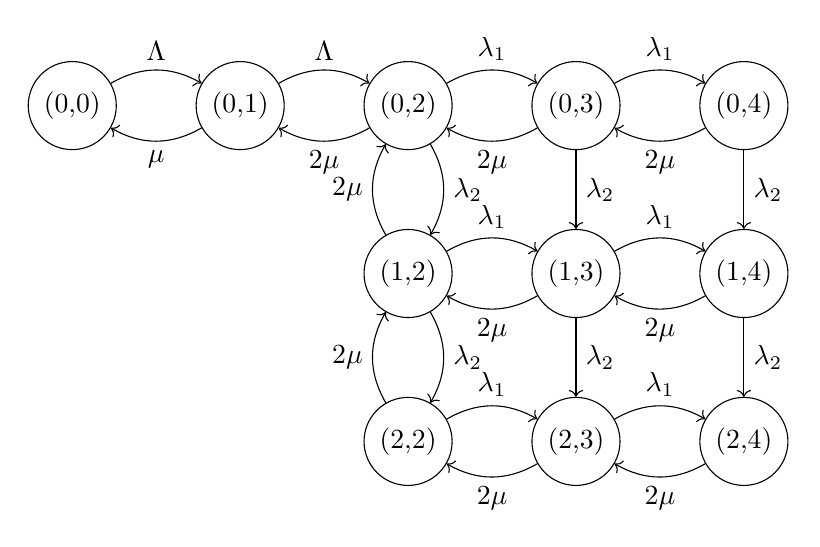
\begin{tikzpicture}[-, node distance = 1cm, auto]
\node[state] (u0v0) {(0,0)};
\node[state, right=of u0v0] (u0v1) {(0,1)};
\draw[->](u0v0) edge[bend left] node {\( \Lambda \)} (u0v1);
\draw[->](u0v1) edge[bend left] node {\(\mu \)} (u0v0);
\node[state, right=of u0v1] (u0v2) {(0,2)};
\draw[->](u0v1) edge[bend left] node {\( \Lambda \)} (u0v2);
\draw[->](u0v2) edge[bend left] node {\(2\mu \)} (u0v1);
\node[state, below=of u0v2] (u1v2) {(1,2)};
\draw[->](u0v2) edge[bend left] node {\( \lambda_2 \)} (u1v2);
\draw[->](u1v2) edge[bend left] node {\(2\mu \)} (u0v2);
\node[state, below=of u1v2] (u2v2) {(2,2)};
\draw[->](u1v2) edge[bend left] node {\( \lambda_2 \)} (u2v2);
\draw[->](u2v2) edge[bend left] node {\(2\mu \)} (u1v2);
\node[state, right=of u0v2] (u0v3) {(0,3)};
\draw[->](u0v2) edge[bend left] node {\( \lambda_1 \)} (u0v3);
\draw[->](u0v3) edge[bend left] node {\(2\mu \)} (u0v2);
\node[state, right=of u1v2] (u1v3) {(1,3)};
\draw[->](u1v2) edge[bend left] node {\( \lambda_1 \)} (u1v3);
\draw[->](u1v3) edge[bend left] node {\(2\mu \)} (u1v2);
\draw[->](u0v3) edge node {\( \lambda_2 \)} (u1v3);
\node[state, right=of u2v2] (u2v3) {(2,3)};
\draw[->](u2v2) edge[bend left] node {\( \lambda_1 \)} (u2v3);
\draw[->](u2v3) edge[bend left] node {\(2\mu \)} (u2v2);
\draw[->](u1v3) edge node {\( \lambda_2 \)} (u2v3);
\node[state, right=of u0v3] (u0v4) {(0,4)};
\draw[->](u0v3) edge[bend left] node {\( \lambda_1 \)} (u0v4);
\draw[->](u0v4) edge[bend left] node {\(2\mu \)} (u0v3);
\node[state, right=of u1v3] (u1v4) {(1,4)};
\draw[->](u1v3) edge[bend left] node {\( \lambda_1 \)} (u1v4);
\draw[->](u1v4) edge[bend left] node {\(2\mu \)} (u1v3);
\draw[->](u0v4) edge node {\( \lambda_2 \)} (u1v4);
\node[state, right=of u2v3] (u2v4) {(2,4)};
\draw[->](u2v3) edge[bend left] node {\( \lambda_1 \)} (u2v4);
\draw[->](u2v4) edge[bend left] node {\(2\mu \)} (u2v3);
\draw[->](u1v4) edge node {\( \lambda_2 \)} (u2v4);
\end{tikzpicture}}
        \caption{Example of Markov chain}
        \label{fig:example-algeb-blocking}
    \end{figure}
    \columnbreak
    \begin{align}
        b(1,2) &= c(1,2) + p_o b(1,3) \label{eq:first_eq_of_blocking_example} \\
        b(1,3) &= c(1,3) + p_s b(1,2) + p_o b(1,4) \\
        b(1,4) &= c(1,4) + b(1,3) \\
        b(2,2) &= c(2,2) + p_s b(1,2) + p_o b(2,3) \\
        b(2,3) &= c(2,3) + p_s b(2,2) + p_o b(1,4) \\
        b(2,4) &= c(2,4) + b(2,3)\label{eq:last_eq_of_blocking_example}
    \end{align}
\end{multicols*}

Additionally, the above equations can be transformed into a linear system of the 
form \(Zx=y\) where:

\begin{equation}\label{eq:example-algebaric-approach-blocking-time}
    Z=
    \begin{pmatrix}
        -1 & p_o & 0 & 0 & 0 & 0 \\ %(1,2)
        p_s & -1 & p_o & 0 & 0 & 0 \\ %(1,3)
        0 & 1 & -1 & 0 & 0 & 0 \\ %(1,4)
        p_s & 0 & 0 & -1 & p_o & 0\\ %(2,2)
        0 & 0 & 0 & p_s & -1 & p_o \\ %(2,3)
        0 & 0 & 0 & 0 & 1 & -1 \\ %(2,4)
    \end{pmatrix},
    x=
    \begin{pmatrix}
        b(1,2) \\
        b(1,3) \\
        b(1,4) \\
        b(2,2) \\
        b(2,3) \\
        b(2,4) \\
    \end{pmatrix}, 
    y=
    \begin{pmatrix}
        -c(1,2) \\
        -c(1,3) \\
        -c(1,4) \\
        -c(2,2) \\
        -c(2,3) \\
        -c(2,4) \\
    \end{pmatrix}
\end{equation}

A more generalised form of the equations in 
(\ref{eq:example-algebaric-approach-blocking-time})
can thus be given for any value of \(C,T,N,M\) by:

\begin{align}
    b(1,T) =& c(1, T) + p_o b(1, T + 1) \label{eq:first_eq_of_blocking_general}\\
    b(1,T + 1) =& c(1, T + 1) + p_s(1, T) + p_o b(1, T + 1) \\
    b(1,T + 2) =& c(1, T + 2) + p_s(1, T + 1) + p_o b(1, T + 3) \\
    & \vdots \nonumber \\
    b(1, N) =& c(1, N) + b(1, N - 1) \\
    b(2, T) =& c(2, T) + p_s b(1, T) + p_o b(2, T + 1) \\
    b(2, T + 1) =& c(2, T + 1) + p_s b(2, T) + p_o b(2, T + 2) \\
    & \vdots \nonumber \\
    b(M, T) =& c(M, T) + b(M, T-1) \label{eq:last_eq_of_blocking_general}
\end{align}

The equivalent matrix form of the linear system of equations 
(\ref{eq:first_eq_of_blocking_general}) - (\ref{eq:last_eq_of_blocking_general})
is given by \(Zx=y\), where:
\begin{equation}\label{eq:general-algebaric-approach-blocking-time}
    \scalebox{0.9}{
        \(
        Z = 
        \begin{pmatrix}
            -1 & p_o & 0 & \dots & 0 & 0 & 0 & 0 & 0 & \dots & 0 & 0 \\ %(1,T)
            p_s & -1 & p_o & \dots & 0 & 0 & 0 & 0 & 0 & \dots & 0 & 0 \\ %(1,T+1)
            0 & p_s & -1 & \dots & 0 & 0 & 0 & 0 & 0 & \dots & 0 & 0 \\ %(1,T+2)
            \vdots & \vdots & \vdots & \ddots & \vdots & \vdots & \vdots & \vdots & 
            \vdots & \ddots & \vdots & \vdots \\ 
            0 & 0 & 0 & \dots & 1 & -1 & 0 & 0 & 0 & \dots & 0 & 0 \\ %(1,N)
            p_s & 0 & 0 & \dots & 0 & 0 & -1 & p_o & 0 & \dots & 0 & 0 \\ %(2,T)
            0 & 0 & 0 & \dots & 0 & 0 & p_s & -1 & p_o & \dots & 0 & 0 \\ %(2,T+1)
            \vdots & \vdots & \vdots & \ddots & \vdots & \vdots & \vdots & \vdots & 
            \vdots & \ddots & \vdots & \vdots \\ 
            0 & 0 & 0 & \dots & 0 & 0 & 0 & 0 & 0 & \dots & 1 & -1 \\ %(M,T)
        \end{pmatrix},
        x = 
        \begin{pmatrix}
            b(1,T) \\
            b(1,T+1) \\
            b(1,T+2) \\
            \vdots \\
            b(1,N) \\
            b(2,T) \\
            b(2,T+1) \\
            \vdots \\
            b(M,T) \\
        \end{pmatrix}, 
        y= 
        \begin{pmatrix}
            -c(1,T) \\
            -c(1,T+1) \\
            -c(1,T+2) \\
            \vdots \\
            -c(1,N) \\
            -c(2,T) \\
            -c(2,T+1) \\
            \vdots \\
            -c(M,T) \\
        \end{pmatrix}
        \)
    }
\end{equation}

Thus, having calculated the mean blocking time for all blocking states \(b(u,v)\), 
it only remains to put them together in a formula.
The resultant blocking time formula is given by:

\begin{equation}\label{eq:algebraic-blocking-time}
    B = \frac{\sum_{(u,v) \in S_A} \pi_{(u,v)} \; b(u,v)}{\sum_{(u,v) \in S_A} 
    \pi_{(u,v)}}
\end{equation}

\subsection{Example}

\newpage
\section{Behavioural Methodology}

\subsection{Backwards Induction}

\subsection{Nash Equilibrium}

\subsection{Learning Algorithms}

\newpage
\section{EMS-ED application}

\subsection{Application}

\subsection{Data analysis of generated problem}

\newpage
\section{Conclusion}



\end{document}